\noindent
\begin{tabular}{cc}
\begin{minipage}{0.45\textwidth}
\begin{exerciseS}[Profili in schiera]
Un numero elevato di profili è disposto come in figura. Il profilo di ingresso
è uniforme $\bm{u} = U_\infty \bm{\hat{x}}$, mentre il profilo di uscita ha andamento
$\bm{u} = \beta U_\infty (\cos \theta \bm{\hat{x}} - \sin \theta \bm{\hat{y}})
\sin{\frac{\pi \eta}{H}}$ in ogni canale (sia $\eta$ la coordinata che descrive la
sezione di uscita).
Sulla sezione di ingresso la pressione media vale $P_1$, sulla sezione di uscita
 $P_2$. 

Calcolare il fattore $\beta$ del profilo di velocità in uscita e la risultante delle
 forze (per unità di apertura) agente sul singolo profilo.

(Risultati: $\beta = \frac{\pi}{2 \cos \theta}, \bm{F} = [(P_1 - P_2) H + \rho U^2 H ((1-\pi^2/8) ]\bm{\hat{x}} + \pi^2/8 \tan \theta \bm{\hat{y}}) $)
\end{exerciseS}
\end{minipage}
&
\begin{minipage}{0.50\textwidth}
   \begin{center}
   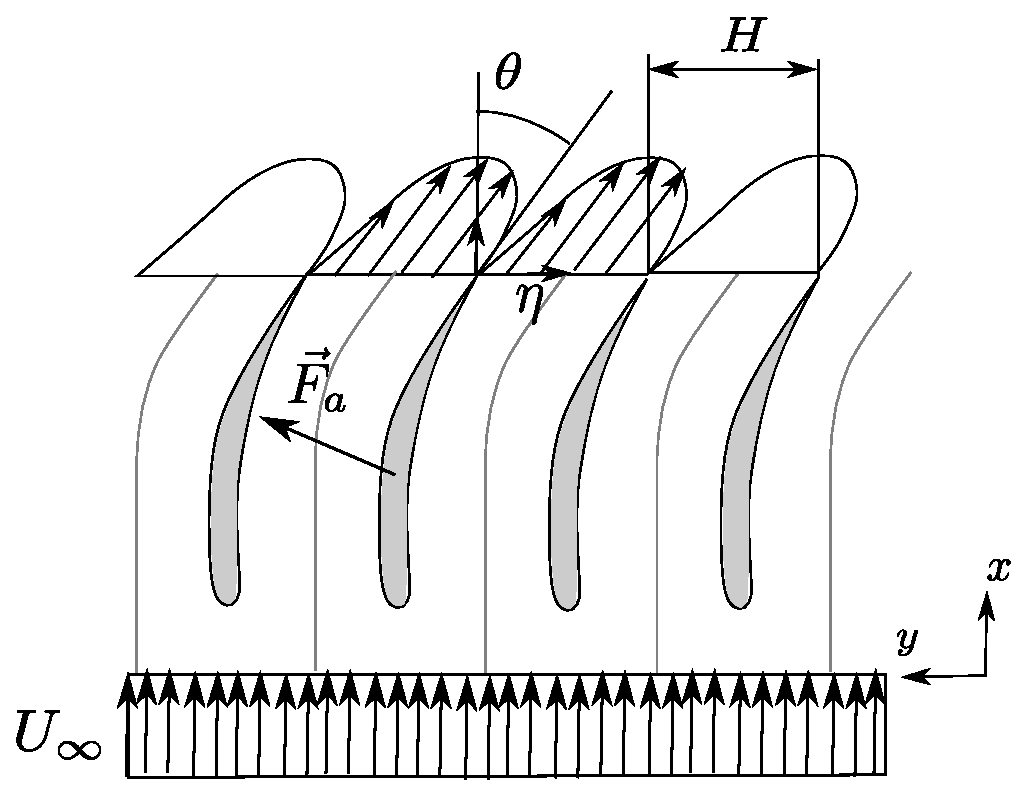
\includegraphics[width=0.95\textwidth]{./fig/wings.eps}
   \end{center}
\end{minipage}
\end{tabular}

\vspace{1.0cm}

\sol

\partone
  Bilanci integrali di massa e quantità di moto. Equazioni di equilibrio (equazioni fondamentali della dinamica classica). Principio di azione e reazione. Integrale della normale su una superficie chiusa è identicamente nullo. Simmetria.
\begin{itemize}
  \item Ricavare il coefficiente $\beta$ dal bilancio di massa
  \item Usare le ipotesi di simmetria nel bilancio di quantità di moto per annullare alcuni termini
\end{itemize} 

\parttwo

Si ricava il coefficiente $\beta$ dal bilancio di massa in forma integrale. Si utilizza la simmetria del problema nel bilancio di quantità moto per
 ricavare le azioni sui profili.

